\chapter{Marco Teórico}

\begin{center}
\begin{minipage}{0.9\textwidth}
{\small
{\bf Resumen:} En el presente capítulo introduciremos la aproximación del Hamiltoniano de enlace fuerte. Utilizando dicha aproximación, presentaremos el modelo Su-Schrieffer-Heeger (SSH) y describiremos la aparición de estados polarizados en dicho modelo; la aparición de dichos estados estará determinada por un invariante topológico llamado \textit{Fase de Berry}. También se discutirá el modelo de Rice-Mele que sustituye los parámetros de salto del modelo SSH por parámetros cíclicos y agrga un parametro de sitio, obteniendo estados de bombeo de carga.
}
\end{minipage}
\end{center}

    
    \section{Modelo de enlace fuerte (TB)}
    El modelo de enlace fuerte (TB, por sus siglas en inglés) es una aproximación semiempírica utilizada para calcular la estructura de bandas electrónica y los estados Bloch de un electrón en un cristal. La aproximación es simple y computacionalmente eficiente por lo que es común utilizarlo para hacer cálculos sobre sistemas muy grandes.
    El modelo, consiste en expandir los estados de un cristal en combinaciones lineales de orbitales localizados tipo atómicos; y así, en dicha base resolver la ecuación de Schrödinger.
    
    Consideremos la ecuación de Schrödinger $H \ket{\psi} = E \ket{\psi}$ de un cristal con un átomo en su celda unitaria, el cual podemos describir por un sólo orbital. El eigenestado de dicho cristal se puede escribir como $\ket{\psi} = \displaystyle 
    \sum_{i} c_i \ket{\omega_i}$, donde $\omega_i(\boldsymbol{r})=\braket{\boldsymbol{r}}{\omega_i}$ es una función tipo orbital localizada del $i$-ésimo sitio tal que $\braket{\omega_i}{\omega_j} = 0$  con $i \neq j$. Los coeficientes $c_i$ se pueden obtener resolviendo el sistema de ecuaciones:
    \begin{equation} 
        \label{eq:Hopping_no_ortogonal}
        \sum_i c_i \sandwich{\omega_i}{H}{\omega_j} = E c_j
    \end{equation}
    
    El modelo de enlace fuerte describe las propiedades de electrones fuertemente ligados a los átomos del cristal, por lo que la interacción entre atómos vecinos decae de tal manera que solo se considera la interacción a vecinos cercanos, en consecuencia  $\sandwich{\omega_i}{H}{\omega_j} = \gamma_{i,j}$ si $i$ y $j$ son átomos vecinos cercanos, donde $\gamma_{i,j}$ se llama integral de salto o {\it hopping} y $\sandwich{\omega_i}{H}{\omega_j} = 0$ si $i$ y $j$ no son vecinos cercanos. Dada la hermiticidad de la matriz el parámetro de {\it hopping} es igual a su complejo conjugado $\gamma_{i,j} = \gamma^*_{j,i}$.

    Ajustamos la energía de referencia tal $\sandwich{\omega_j}{H}{\omega_j} = 0$. Entonces, la ecuación \ref{eq:Hopping_no_ortogonal} esta dada por:

    \begin{equation}
        \sum_{\langle i, j \rangle } ( \gamma_{i,j} - \delta_{i,j}E )c_j = 0, \,\,\, \forall\,\, j
    \end{equation}
    
    
    % --- Párrafo cambiado por el anterior
    % Las suposiciones que convierten a este modelo en un modelo de amarre fuerte consisten en suponer que la interacción entre los átomos decae de tal manera que solo se considera la interacción a primeros vecinos, entonces  $\sandwich{\phi_i}{H}{\phi_j} = \gamma_{i,j} = \gamma*_{j,i}$, donde a $\gamma_{i,j}$ se le conoce como parametro de \textit{hopping}, dado que se pide la condición de igualdad de el parámetro de hopping con su complejo conjugado, se obtiene una matriz Hermitiana, por lo que para $i = j$ tenemos $\sandwich{\phi_j}{H}{\phi_j} = 0$ . Entonces, la ecuación \ref{Coefficent_no_ortogonal} se convierte en:
    % \begin{equation}
    %     \sum_{\langle i, j \rangle } ( \gamma_{i,j} - \delta_{i,j}E )c_j = 0, \,\,\, \forall\,\, j
    % \end{equation}
    %%%%%%%%%% 
    
    
    Con esto hemos convertido el problema de la solución de la ecuación de Schrödinger en un problema de eigenvalores para un matriz (ver~\ref{SecEjemplo} Ejemplo).
    %de $i\times j$, para valores pequeños de $i $ y $j$ esta matriz se puede sencillamente (ver ejemplo)  para valores mas grandes esta matriz se puede diagonalizar de manera numérica.

    \subsection{Ejemplo}
    \label{SecEjemplo}
    \vspace{-1.5cm}

    \begin{figure}[h!]
        \centering
        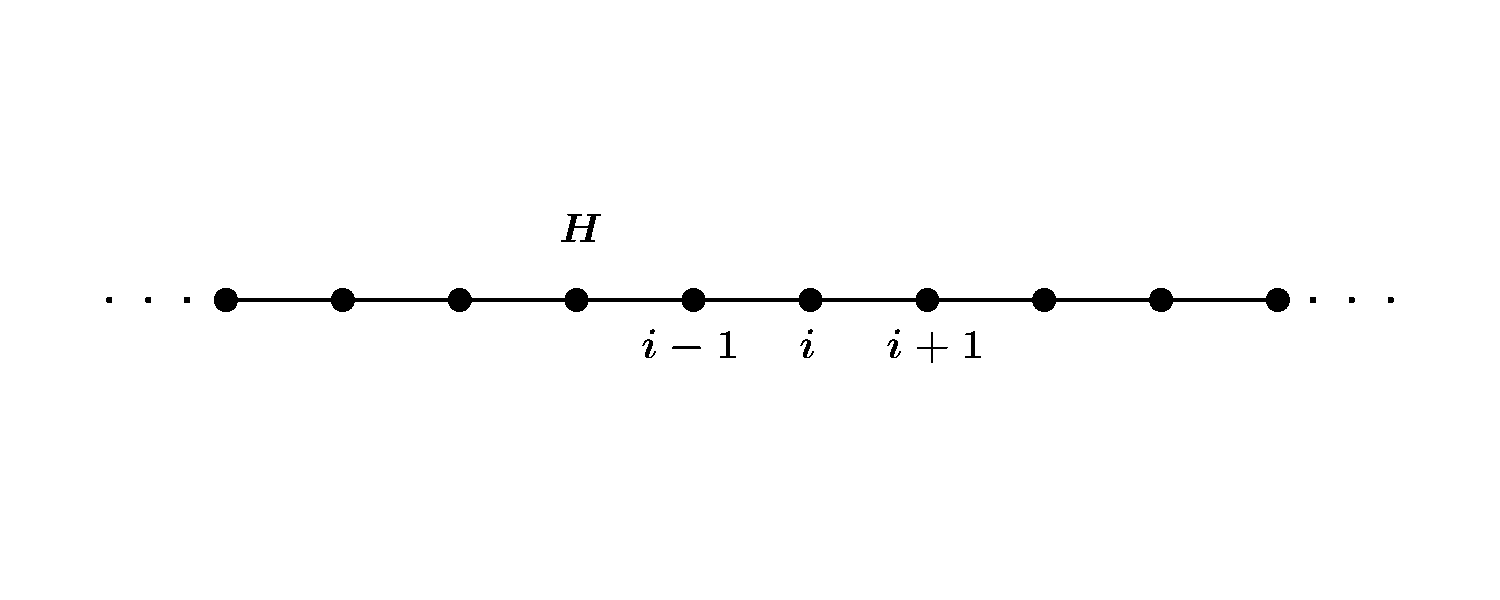
\includegraphics[width=\textwidth]{Imagenes/Models/TB_example.pdf}\vspace{-1.5cm}
        \caption{Red cristalina unidimensional de átomos de hidrogeno}
        \label{fig:Hidrogen_chain}
    \end{figure}
    
    Supongamos que tenemos una red unidimensional cristalina de átomo de hidrogeno que se acomodan sobre una línea recta, como se muestra en la figura(\ref{fig:Hidrogen_chain}). Los traslapes de los orbitales localizados entre vecinos cercanos ayudan al electrón a deslocalizarse de una celda a otra, saltando de un átomo a otro, este potencial de salto está dado por el potencial de traslape o \textit{hopping} entre dos sitios, denotado por $\gamma_{i,j}$, para este sistema el hamitoniano de amarre fuerte está dado por:

    \begin{equation}
        \label{HidrogenoTBH}
        H =  -\sum_{i}\sum_{\langle i, j \rangle } \gamma_{ij} \ket{i}\bra{j}
    \end{equation}
    donde la primera suma es sobre el índice de la celda y la segunda suma es sobre los vecinos cercanos del átomo en la celda unitaria.
    
    Dado que tenemos un sistema periódico, empezaremos escribiendo el operador de traslación $T = \ket{i}\bra{i+1}$ el cual denota la traslación del sitio $i$ al $i+1$, si asumimos que los términos de {\it hopping} dependen únicamente de la distancia entre dos sitios, entonces, $\gamma_{i,i+n} \equiv \gamma_{n}$, entonces ahora podemos escribir el Hamiltoniano de la ecuación \ref{HidrogenoTBH} en función del operador de traslación como $H = -\sum_n \gamma_n T_n$, notemos que ahora es posible diagonalizar el hamiltoniano en la base del operador de traslación, la cual sabemos esta compuesta por los estados de onda plana definidas como:

    \begin{equation}
        \ket{k} = \frac{1}{\sqrt{N}} \sum_j e^{ikj} \ket{j} 
    \end{equation}
    con $k \in \{-\pi/a\,,\,\pi/a\}$.
    
    Si vemos la acción del operador $T^n$ sobre $\ket{k}$ tenemos $T^n \ket{k} =  e^{-ikna}\ket{k}$ 
    por lo tanto la solución al espectro de energías de la ecuación $H(k)\ket{k} = E(k)\ket{k}$, recordando que solo se toma la interacción a primeros vecinos, esta dada por:
    \begin{equation}
        E(k) = 2\gamma \cos(ka)
    \end{equation}
    
\section{Modelo Su-Schrieffer-Heeger (SSH)}
    

El modelo de Su-Schrieffer-Heeger (SSH) es un modelo de amarre fuerte (TB) que describe un electrón sin espín en una celda unitaria con dos sitios en un red unidimensional, un sitio etiquetado por $A$ y otro por $B$ (fig \ref{fig:SSH_Fig}). Las interacciones entre los electrones no son consideradas y la dinámica de los electrones esta descrita por el Hamiltoniano de una sola partícula (\ref{eq:Hamiltonian_ssh}).

\begin{figure}[h!]
    \centering
    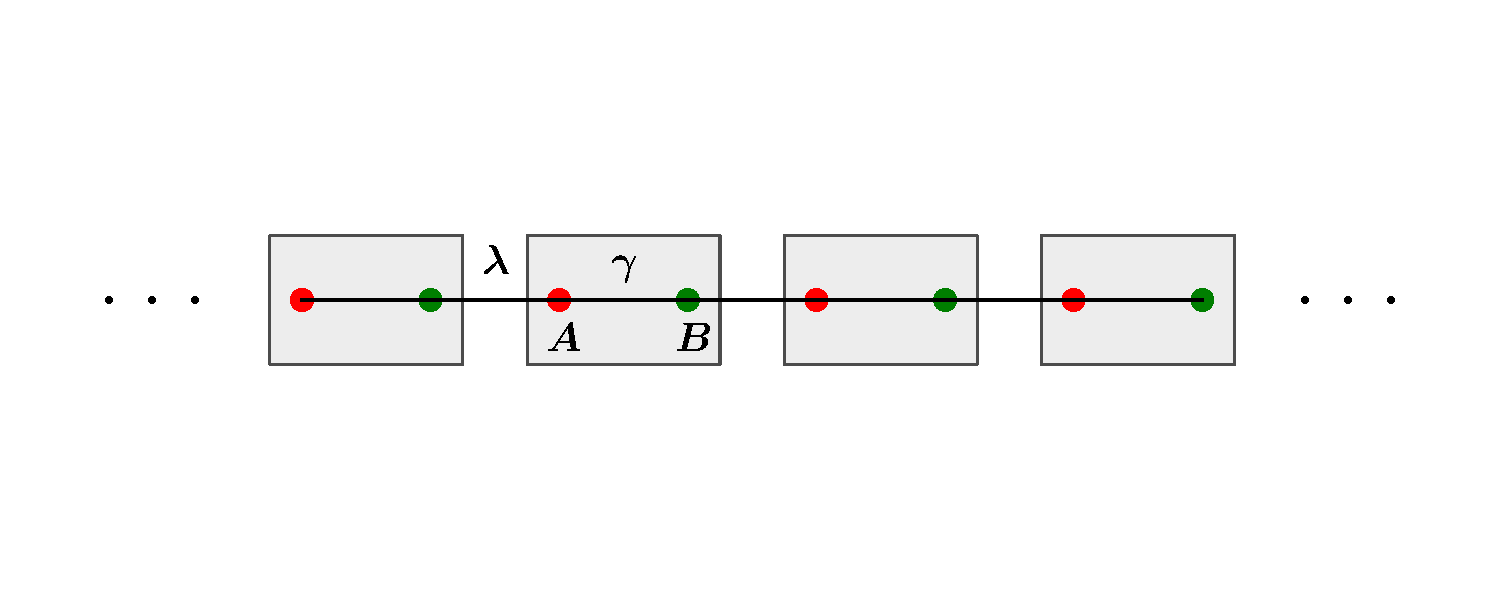
\includegraphics[width=\textwidth]{Imagenes/Models/SSH_example.pdf}\vspace{-1.5cm}
    \caption{Modelo SSH para una cadena de poliacetileno, con una calda unitaria conformada por dos sitios $A$ y $B$, conectadas por parametros de salto intracelda ($\gamma$) e intercelda ($\lambda$)}
    \label{fig:SSH_Fig}
\end{figure}


\begin{equation}
    \label{eq:Hamiltonian_ssh}
    H = \gamma \sum_{i=1}^N (\ket{i,A}\bra{i,B} \,+\, h.c. ) + \lambda \sum_{i=1}^{N-1} (\ket{i + 1,A}\bra{i,B} \,+\, h.c. ) 
\end{equation}

Donde $\bra{i,A}$ y $\bra{i,B}$ denotan el estado de la cadena donde el electrón se encuentra en el i-sima celda , con $i \in {1,2,...,N}$ y en el sitio $A$ o $B$, respectivamente. El parametro de salto intracelda esta dado por $\gamma$ y el intertcelda por $\gamma$. El sumando $h.c.$ representa el hermitiano conjugado.

La matriz del modelo SSH para una cadena con $N = 4$ celdas unitarias en el espacio real, se ve como la ecuación \ref{eq:Hamiltonian_ssh_real}.

\begin{equation}
    \label{eq:Hamiltonian_ssh_real}
    H = 
     \begin{pmatrix}
            0 & \gamma & 0 & 0 & 0 & 0 & 0 & 0 \\
            \gamma & 0 & \lambda & 0 & 0 & 0 & 0 & 0 \\
            0 & \lambda & 0 & \gamma & 0 & 0 & 0 & 0 \\
            0 & 0 & \gamma & 0 & \lambda & 0 & 0 & 0 \\
            0 & 0 & 0 & \lambda & 0 & \gamma & 0 & 0 \\
            0 & 0 & 0 & 0 & \gamma & 0 & \lambda & 0 \\
            0 & 0 & 0 & 0 & 0 & \lambda & 0 & \gamma \\
            0 & 0 & 0 & 0 & 0 & 0 & \gamma & 0 \\
            
        \end{pmatrix}
\end{equation}

Suponiendo que nuestro sistema tiene periodicidad posicional, podemos utilizar el teorema de Bloch $\Psi_{n,k}(\mathbf{r}) = e^{i k\mathbf{r}} u_{n,k}(\mathbf{r})$ con:
\begin{equation}
    H(k + 2\pi) = H(k) ; \,\,\,\,\,\,\,\, \ket{u(k + 2\pi)} = \ket{u(k)} 
\end{equation}


de tal forma que la ecuación de Shrödringer definida por el hamiltoniano escrito en el espacio de momentos para el cuerpo de la cadena, esta dado por:

\begin{equation}
    \label{eq:Hamiltonian_ssh_bloch}
    H =      
     \begin{pmatrix}
            0 & \gamma + \lambda e^{-ik}  \\
            \gamma + \lambda e^{ik} & 0  \\
        \end{pmatrix} ; \,\,\,\, H(k) \begin{pmatrix}
            a(k)   \\
            b(k)  \\
        \end{pmatrix} = E(k) \begin{pmatrix}
            a(k)   \\
            b(k)  \\
        \end{pmatrix}
\end{equation}

Esta forma simplifica mucho el calculo de los invariantes topológicos que definen los estados electrónicos de estos aislantes topológicos.


\begin{figure}[h!]
     \centering
    \captionsetup[sub]{font=small}

     \begin{subfigure}[b!]{0.27 \textwidth}
         \caption{}
         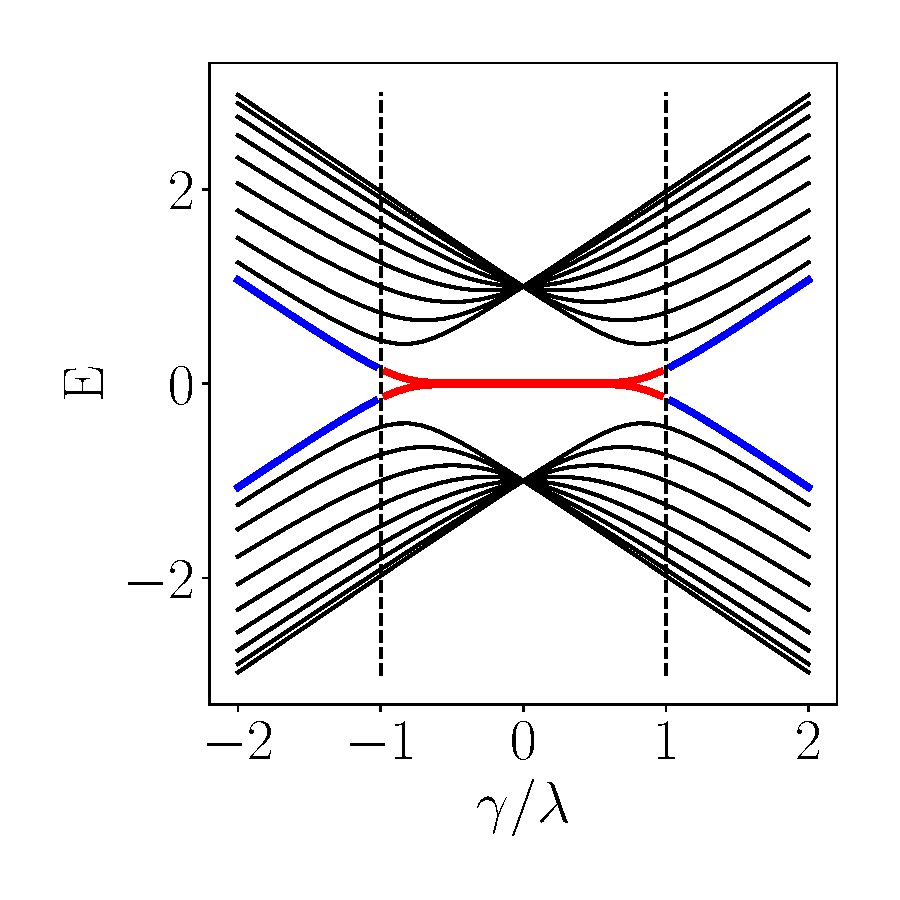
\includegraphics[width=\textwidth]{Imagenes/Shh_images/bands_shh.pdf}
     \end{subfigure}\hspace*{-0.9em}
     \begin{subfigure}[b!]{0.27 \textwidth}
         \caption{}
         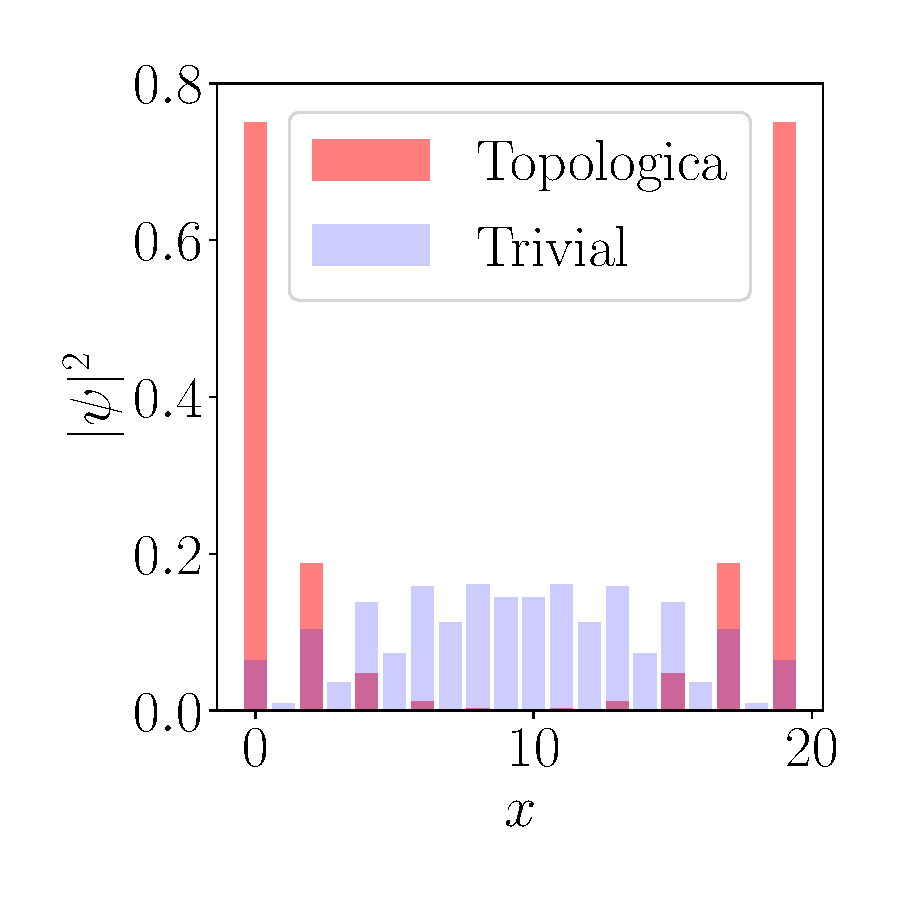
\includegraphics[width=\textwidth]{Imagenes/Shh_images/proyection_ssh.pdf}
     \end{subfigure}\hspace*{-0.9em}
     \begin{subfigure}[b!]{0.27 \textwidth}
         \caption{}
         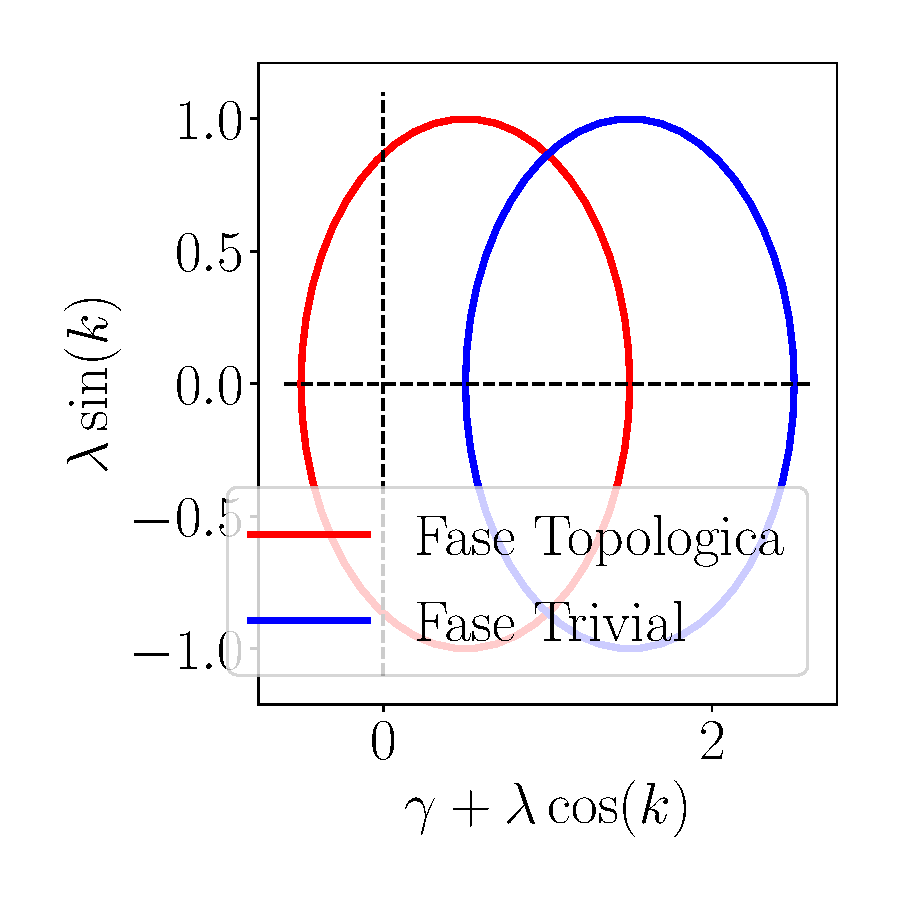
\includegraphics[width=\textwidth]{Imagenes/Shh_images/loop_shh.pdf}
     \end{subfigure}\hspace*{-0.9em}
     \begin{subfigure}[b!]{0.27 \textwidth}
         \caption{}
         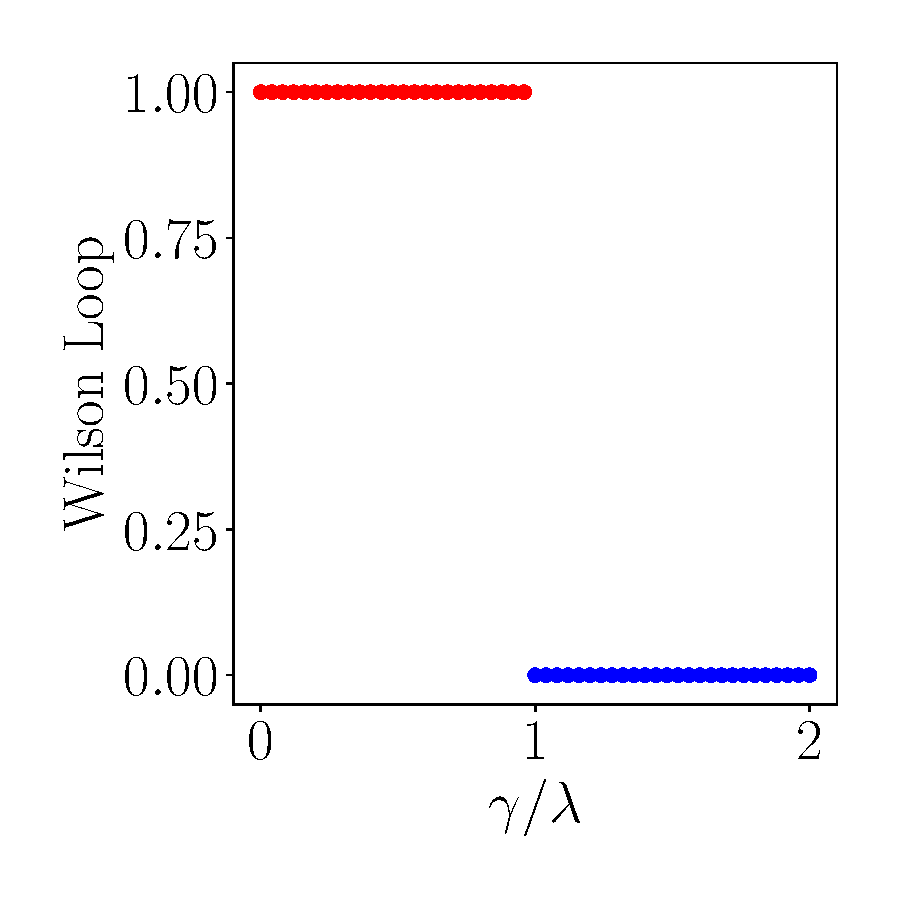
\includegraphics[width=\textwidth]{Imagenes/Shh_images/winding_shh.pdf}
     \end{subfigure}
        \caption{\textbf{(a)} Variación del espectro de energias conforme cambian los parámetros de salto $\gamma/\lambda$. \textbf{(b)} Proyección de la densidad de probabilidad de los estados de borde en la fase topológica (rojo) y en la fase trivial (azul). \textbf{(c)} Representación grafica del número de Winding con valor $1$ en fase topológica (rojo) y $0$ en la fase trivial (azul). \textbf{(d)} Fase de Berry dependiente de los parametros de salto $\gamma/\lambda$ con valor $1$ en fase topológica (rojo) y $0$ en la fase trivial (azul)}.
        \label{fig:SSH_Img_Results}
\end{figure}

Al resolver el sistema de los hamiltonianos (\ref{eq:Hamiltonian_ssh_real}) y (\ref{eq:Hamiltonian_ssh_bloch}) obtenemos los resultados de la figura (\ref{fig:SSH_Img_Results}), en \textbf{(a)} tenemos el comportamiento del espectro de energías conforme los parámetros de salto cambian, las lineas negras corresponden a las energías del cuerpo o bulto de la cadena y las lineas rojas con azul muestran las energías de borde que aparecen debido a la finitud de la cadena y son las energias mas cercanas a la energia de Fermi, Notemos que para los parametros de salto $|\gamma/\lambda|<1$ las energías de los estados de borde se localizan en la energía de Fermi, a estos estados se le conoce como estados topológicos o fase topológica, al proyectar la densidad de probabilidad de los estados correspondientes a estas energías en el espacio real (fig \ref{fig:SSH_Img_Results} \textbf{(b)}), obtenemos para el los parámetros entre los que $\gamma/\lambda < 1$ tenemos la densidad principalmente concentrada en los extremos del material, lo que indicaría un estado de polarización de la cadena, por otro lado, para el los parámetros $|\gamma/\lambda| > 1$ se puede ver en la proyección de los estados de borde la densidad de probabilidad esta distribuida uniformemente en la cadena, como un aislante común, a este estado se le conoce como fase trivial.

Una forma de estudiar el comportamiento de los estados topológicos y triviales de esta cadena, es a través de la información que se puede obtener de la relación de dispersión. 

Supongamos que el hamiltoniano de Bloch de nuestro modelo se puede escribir como una combinación lineal de las matrices de Pauli:

\begin{equation}
    H(k) = d_0(k) \hat{\sigma_0} + d_x(k) \hat{\sigma_x} + d_y(k) \hat{\sigma_y} + d_z(k) \hat{\sigma_z} = d_0(k) \hat{\sigma_0} + \mathbf{d_0}(k) \mathbf{\hat{\sigma_0}}
\end{equation}

Para el modelo SSH, tenemos que:
\begin{equation}
  d_0(k) = 0 ,\; d_x(k) = \gamma + \lambda \cos(k) , \; d_y(k) = \lambda \sin(k), \; d_z(k) = 0  
\end{equation}

La estructura interna de los estados con momento $k$ esta dada por la dirección del vector $\mathbf{d}(k)$, como el numero de onda $k  \in \left[ 0, \; 2\pi \right]$, la ruta que traza $\mathbf{d}(k)$ es un circuito cerrado de radio $\lambda$ en el plano $dx, \,dy$ y centrado en el punto $(\gamma, 0)$. Para que este hamiltoniano describa un aislante es necesario que los círculos que se forman no incluyan el origen\cite{Asboth2015}. La topología de estos ciclos pueden ser caracterizados por un entero, que cuenta el numero de veces que el ciclo rodea el origen, esta cantidad es conocida como el numero de Winding, que es un invariante topológico.

Para el modelo SSH el numero de Winding puede ser 0 o 1, dependiendo de los parámetros, como se puede ver en la \ref{fig:SSH_Img_Results} \textbf{(c)}, donde se puede notar mas a detalle como los ciclos encierran o no el origen dependiendo de los parametros, cambiando las el estado del material entre topológico (rojo) y el trivial (azul). Sin embargo el numero de Winding no es el único numero que caracteriza la topología de la cadena de poliacetileno, en la figura \ref{fig:SSH_Img_Results} \textbf{(d)} se puede observar el comportamiento de la fase de Zak o fase de Berry, que es un invariante topológico que surge de la observación del cambio de fase de la funciones de bloch conforme se recorre de manera cíclica la zona de Brillouin. Este invariante describe como los estados, cuando son topologicos, ganan una fase de $\pi$, es decir, los estados no regresan a su estado inicial después de un ciclo. La Fase de Zak como otros invariantes, es un caso particular de la fase de Berry.

\section{Invariantes topológicos (Fase de Berry)}

Se le llama Invariante topológico a cualquier numero que caracterice a el hamiltoniano de un aislante y que no cambie a través de variaciones adiabáticas. Como consecuencia de estará variaciones el invariante topológico cumple con dos características claves:
\begin{itemize}
    \item Solo esta bien definido en el limite termodinámico.
    \item Depende de las simetrías que se tengan que respetar.
\end{itemize}

Donde se entiende por variación adiabática que los parámetros cambian de forma continua , las simetrías mas importantes del sistema se mantienen y que el gap del bulto o cuerpo de la geometría que están cerca de las energías $E=0$ permanezca abierto.

Existe un gran numero de invariantes topológicos que caracterizan diferentes propiedades físicas de las estructuras geométricas de los materiales, por ejemplo: el numero de Winding, la cantidad de estados de borde, el Willson loop, el numero de Chern, la fase de Berry, etc. Para los fines de este trabajo hablaremos de la fase de Berry, la cual recientemente a sido asociada como responsable de una gran gamma de fenómenos interesantes en las propiedades de los materiales, tales como la ferroelectricidad, el magnetismo orbital, el efecto hall cuantico, el bombeo de cargas y la polarización.

En mecánica cuántica la función de onda normalmente se define con una fase que no tiene sentido físico ya que desaparece al tomar el valor de expectación. Sin embargo la fase de Berry mostró en 1984 que esta fase tiene efectos físicos observables si el sistema se transforma de manera adiabática y cíclica. En ausencia de degeneración, el sistema regresara este mismo punto al cerrar el ciclo, pero habrá una diferencia de fase igual a la integral temporal de la energía mas un termino extra que es lo que conocemos como fase de Berry.

Consideremos un sistema general descrito por el hamiltoniano $H(\mathbf{\lambda})$, donde $\mathbf{\lambda}$ es un conjunto de parámetros que evolucionan en el tiempo, $\mathbf{\lambda} = \left( \lambda_1(t), \lambda_2(t),\dots, \lambda_n(t)\right)$. Tambien introduciomos una base ortonormal de estados en cada punto de $\lambda$ del espacio, $\ket{n(\lambda(t))} = \ket{n(\lambda)}$, tal que:
\begin{equation}
    H(\lambda) \ket{n(\lambda)} =  E_n\ket{n(\lambda)}
\end{equation}
De acuerdo con el teorema adiabatico, un sistema que se encuentra inicialmenten en el estado $\ket{n(\lambda_0)}$ permanecera como un eigenestado instantaneo de $H(\lambda)$ para todo $t$, entonces:
\begin{align}
    \ket{\psi(t)} =  e^{i\theta_n(t)}\ket{n(\lambda)}
\end{align}

Introduciendo la ecuacion anterior en la ecuacion de Shrodringer:
\begin{align}
    (H(\lambda) - \partial_t) e^{i\theta_n(t)}\ket{n(\lambda)} =  0
\end{align}

Desarrollando es fácil obtener la ecuación diferencial para $\theta$:

\begin{align}
    \dot{\theta} = \frac{1}{\hbar} E_n(\lambda) - i \sandwich{n(\lambda)}{\partial_t}{n(\lambda)}
\end{align}

La expresion final para la fase se obtiene integrando en el tiempo:

\begin{align}
   \theta = \frac{1}{\hbar} \int_t E_n(\lambda) d\lambda - i \int_t \sandwich{n(\lambda)}{\partial_t}{n(\lambda)} d\lambda
\end{align}

Notemos que el primer sumando es la fase dinámica usual, mientras el segundo termino es denominado como la fase de Berry:
\begin{align}
    \gamma := i \int_{\lambda(0)}^{\lambda(t)} \sandwich{n(\lambda)}{\partial_\lambda}{n(\lambda)} d\lambda
\end{align}

Donde el termino $A_n = \sandwich{n(\lambda)}{\partial_\lambda}{n(\lambda)}$ es conocido como la conexión de Berry. Si usamos el Teorema de Stokes, si integramos sobre una superficie cerrada $C$ que se puede parametrizar en el tiempo:

\begin{align}
    \gamma_n = \oint_C A_n \cdot d\lambda = \int_S \nabla_\lambda \times A_n \cdot dS_\lambda
\end{align}


Donde al vector $\Omega_n = \nabla_\lambda \times A_n$ se le conoce como curvatura de Berry. Se sabe que la integral de la curvatura de Berry sobre un superficie cerrada, tal como un esfera o un toro, es topológica y esta cuantizada; a estos números cuánticos topológicos se les denomina números de Chern.

\subsection{Polarización, centros de Wannier y Fase de Berry}

En los textos de electromagnetismo la polarización macroscópica se define como la cantidad de dipolos eléctricos por unidad de volumen, donde los dipolos son pequeñas unidades polarizadas, en la simplificación del problema se asume que la distribución de carga entre los dipolos eléctricos es nula. Sin embargo, al estudiar la densidad electrónica de un material polarizado a través de la mecánica cuántica podremos notar que la carga no esta divida en paquetes convenientes y que la unidad de polarización no existe. 

\begin{figure}[tbh!]
    \centering
   \captionsetup[sub]{font=small}
    \begin{minipage}[h!]{1\textwidth}
        \begin{subfigure}[b!]{1 \textwidth}
            \caption{}
            \vspace*{-2em}
            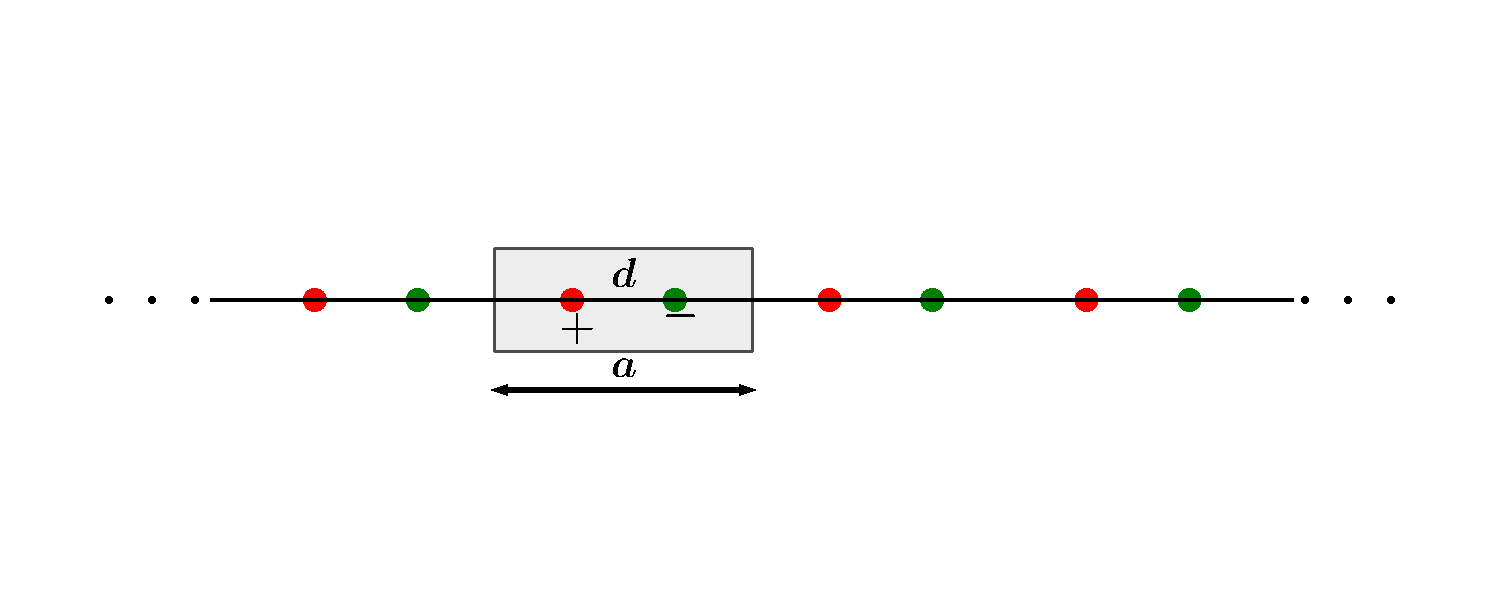
\includegraphics[width=\textwidth]{Imagenes/Models/polarizatio_example_a.pdf}
        \end{subfigure}\hspace*{-0.5em}
    \end{minipage}\vspace*{-2.5em}

    \begin{minipage}[h!]{1\textwidth}
        \begin{subfigure}[b!]{1 \textwidth}
            \caption{}
            \vspace*{-2em}
            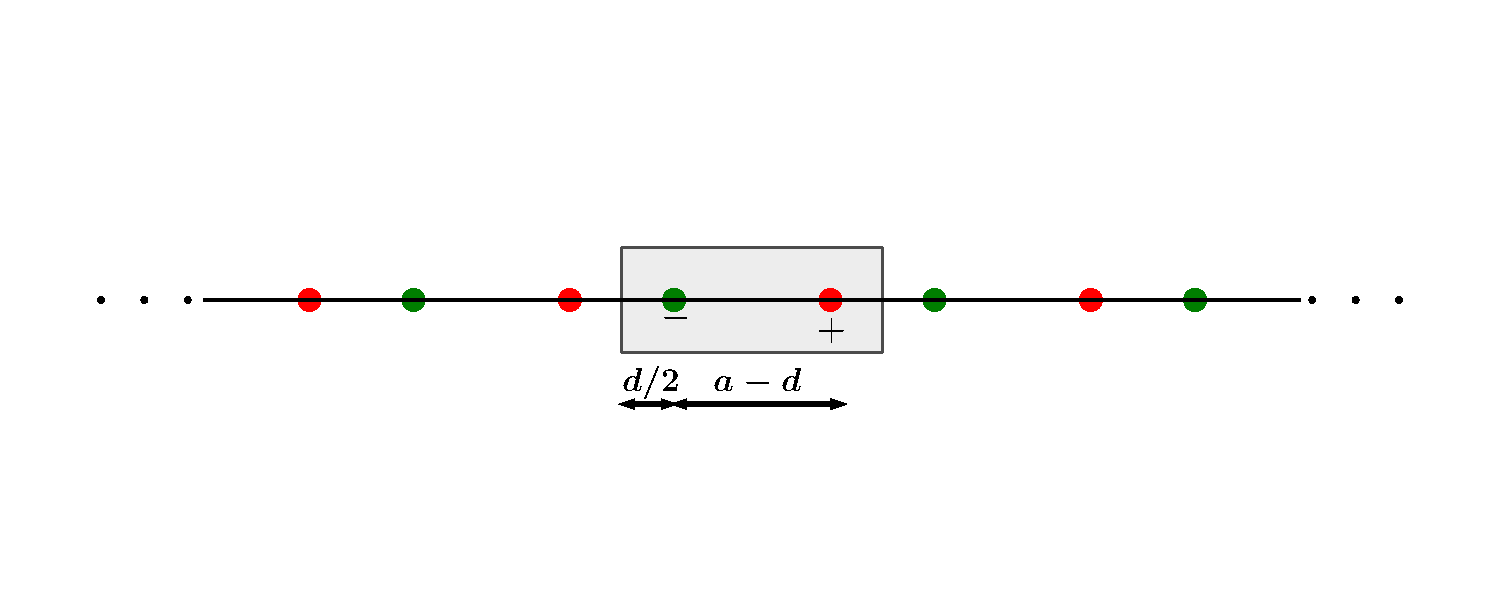
\includegraphics[width=\textwidth]{Imagenes/Models/polarizatio_example_b.pdf}
        \end{subfigure}\hspace*{-0.5em}
    \end{minipage}\vspace*{-1.5em}
    
    \caption{Red cristalina infinita periódica conformada por una molécula dicotómica anión (verde), catión (rojo), separados por una distancia \textbf{(a)} $d$ o \textbf{(b)} $a-d$, dependiendo la elección de celda.}
    \label{fig:Model_polarization}
\end{figure}

Una aparente solución podría ser contar los momentos dipolares como una integral continua sobre la densidad electrónica, sin embargo esta solución es solo aparente, pues esta cantidad depende de como se seleccione la celda sobre la cual se integra, este detalle podría darnos cantidades distintas para para diferentes elecciones de celda, es decir, conocer la densidad electrónica no es información suficiente para determinar la polarización en una red aislante cristalina.
\begin{equation}
\label{polarization_classic}
\textbf{P} = \frac{1}{V_{cell}}\int_{cell} \textbf{r} \rho(\textbf{r})d^3r
\end{equation}

por ejemplo:

Supongamos que tenemos una red cristalina periódica conformada por una molécula dicotómica que se repite indefinidamente formando una cadena infinita, la molécula esta formada por un anión y un catión, ambos separados a una distancia $d$ y la celda unitaria tiene una distancia $a$ (fig \ref{fig:Model_polarization} \textbf{(a)}). Si calculamos la polarización con la expresión \ref{polarization_classic} obtendremos la ecuación \ref{eq:pol1}.

\begin{equation}
    \label{eq:pol1}
    P_1 = \frac{qd}{a}
\end{equation}

Ahora supongamos que la selección de la celda unitaria es de la misma longitud pero con una posición diferente, como se muestra en la (fig \ref{fig:Model_polarization} \textbf{(b)}), al calcular la polarización obtenemos la ecuación \ref{eq:pol2}.

\begin{equation}
    \label{eq:pol2}
    P_2 = \frac{qd}{a} + q
\end{equation}

Si nos tomamos todas las posibles elecciones de celdas llegaremos a la conclusión de que la expresión en general de la polarización estara dada por las expresiones \ref{eq:pol_gral1d} y \ref{eq:pol_gral3d}.

\begin{equation}
    \label{eq:pol_gral1d}
    P = P_o + nq\,\,  {\rm con} \,\,n \in \mathbb{Z}\,\, \text{para el caso 1D} 
\end{equation}

\begin{equation}
    \label{eq:pol_gral3d}
    P = P_o + n\frac{qR}{V}\,\,  \text{con} \,\,n \in \mathbb{Z}\,\, \text{para el caso 3D}
\end{equation}

Donde $P_o$ es la polarización electrónica cuando se escoge convenientemente una celda centrosimétrica, $q$ es la carga de los iones, $R$ es la magnitud del vector de la celda y V es el volumen de la celda.

Como podemos notar, la polarización está multivaluada para diferentes elecciones de celda, donde la polarización difiere entre si en un termino $P_q = \frac{qR}{V}$ el cual es conocido como \textit{``cuanto de polarización''}.

¿Pero que significa esta cantidad? Imaginemos que en nuestro sistema se mueve un electrón de un anión de una celda a otra, ¿Cómo cambia la polarización debido al transporte de carga? La respuesta es $\Delta P = \frac{-ea}{V}$, es decir, como consecuencia de la periodicidad del sistema, el mover un electrón de una celda a otra deja a el sistema físico exactamente igual, pero a la polarización no.

Veamos entonces un ejemplo de transporte de carga. Supongamos una evolución adiabática en el cuerpo de un aislante cristalino, donde el cambio de la polarización estará dado por:

\begin{equation}
    \Delta \textbf{P} = \int_i^f \textbf{J}(t)dt
\end{equation}
Si \textbf{P} estuviera únicamente definida para cualquier ciclo cerrado, implicaría que  $\Delta \textbf{P} = 0$. Ahora supongamos que tenemos una onda de densidad de carga que se desliza por un aislante cristalino uni-dimensional, el hamiltoniano de este modelo está dado por:
\begin{equation}
    H =  \frac{p^2}{2m} - V_0 cos(\frac{2\pi x}{a} - \lambda)
\end{equation}
Donde $a$ es la constante de la red y $\lambda$ es un parámetro de ciclo el cual varia con el tiempo y corre de $0$ a $2\pi$. 
Supongamos que $V_o$ es suficientemente grande para contener a una partícula semiclásica con carga $-e$ atrapada en el potencial al rededor de el mínimo del potencial ($x = \frac{a\lambda}{2\pi}$). Después de un ciclo, la partícula será bombeada de tal forma que:

\begin{equation}
    \Delta \textbf{P}_{cyc} = \oint \textbf{J}(t)dt = -e
\end{equation}

Por lo tanto el bombeo de la carga es inconsistente con la idea de que la polarización es únicamente  definida. 

Pero ahora ¿Como calculamos esta diferencia de polarización para casos donde las cargas no están localizadas como sucede en los sistemas cuánticos cristalinos donde la carga esta distribuida por todo el cristal? Primero debemos notar que la contribución de los electrones a la polarización es una propiedades del estado electrónico de varios cuerpos, la idea central para contestar esta pregunta es escribir estos estados electrónicos de varios cuerpos usando una base ortonormal  de estados localizados que nos permitan tener una visualización tipo átomo de la densidad electrónica, que comúnmente es una función continua en todo el espació, esta descripción nos permitirá seguir sumando los momentos dipolares como cargas multiplicadas por sus posiciones. La base de estados que permitirá todo esto es conicidad estados de Wannier. La contribución de cada electrón en un estado Wannier al centro de carga puede evaluarse fácilmente y luego sumarse.

Las funciones de Wannier $w_n(\textbf{r})$ de la n-sima banda, en la celda unitaria asociada a $\textbf{R}$, están definidas como:
\begin{equation}
\begin{split}
     w_n(\textbf{r} - \textbf{R}) &= \frac{\Omega}{(2\pi)^3} \int_{BZ} d^3\textbf{k} e^{-i \textbf{k} \cdot \textbf{R}} \Psi_{n\textbf{k}}(\textbf{r})\\
     &= \frac{\Omega}{(2\pi)^3} \int_{BZ} d^3\textbf{k} e^{i \textbf{k} \cdot (\textbf{r} - \textbf{R})} u_{n\textbf{k}}(\textbf{r})
\end{split}
\end{equation}

A diferencia de las funciones de Bloch que están deslocalizadas en el espacio las funciones de Wannier si están localizadas. Estás son relevantes para este problema porque la naturaleza de la localización proporciona una conveniente descripción de la densidad de carga en un sólido. Si bien sabemos en
realidad de que la densidad de carga en un sólido es una función continua, la idea de que esta puede estar localizada nos permitirá continuar calculando los momentos dipolares sumando sobre cargas multiplicadas por posiciones (Ahora tenemos una manera conveniente de tomar las celdas que permitan esto).
Para esto primero suponemos que la concentración de electrones esta al rededor de la función de Wannier, a esta "posición" de la función de wannier se les llama ``Centros de Wannier", $\overline{\textbf{r}}$ y se calcula como el valor esperado de la posición:
\begin{equation}
\label{eq:Wcenter}
\begin{split}
        \overline{\textbf{r}} &= \sandwich{w_n}{\textbf{r}}{w_n}\\
        &= \int w^*_n(\textbf{r})\,\textbf{r}\, w_n(\textbf{r})\, d^3\textbf{r}
\end{split}
\end{equation}
Como se verá más adelante en el marco teórico, la ecuación \ref{Wcenter} se puede escribir en términos de las funciones periódicas $u_{n\textbf{k}}$ y usando al operador posición en la representación de momentos $\textbf{r} = -i\frac{\partial}{\partial\textbf{k}}$:
\begin{equation}
    \overline{\textbf{r}} = i\frac{\Omega}{(2\pi)^3} \int_{BZ} d^3\textbf{k}\,e^{-i\textbf{k}\cdot\textbf{R}}\braket{u_{n\textbf{k}}}{\frac{\partial u_{n\textbf{k}} }{\partial\textbf{k}}}
\end{equation}

Con el concepto de los centros de Wannier, ahora, la expresión para la polarización se puede escribir como las contribuciones de los iones (ya antes localizados) y las contribuciones debido a las cargas electrónicas centradas, ahora, en los centros de Wannier, para cada banda ocupada.

\begin{equation}
    p = \frac{1}{V_{cell}} (\sum_i (q_i x_i)^{ions} + \sum_n^{occ}(q_n \overline{\textbf{r}})^{WF})
\end{equation}

Es importante recalcar que el segundo termino en la polarización es mejor conocido como como la fase de Berry:
\begin{equation}
    \label{eq:Barry_fase}
    \sum_n^{occ}\int_{BZ} d^3\textbf{k}\,e^{-i\textbf{k}\cdot\textbf{R}}\braket{u_{n\textbf{k}}}{\frac{\partial u_{n\textbf{k}} }{\partial\textbf{k}}}
\end{equation}
Está cantidad será la central en el calculo de invariantes topológicos en estados de polarización que definen a un aislante topológico de alto orden. 


\section{Bombeo Adiabático}

\begin{figure}[h!]
     \centering
    \captionsetup[sub]{font=small}

     \begin{subfigure}[b!]{0.27 \textwidth}
         \caption{}
         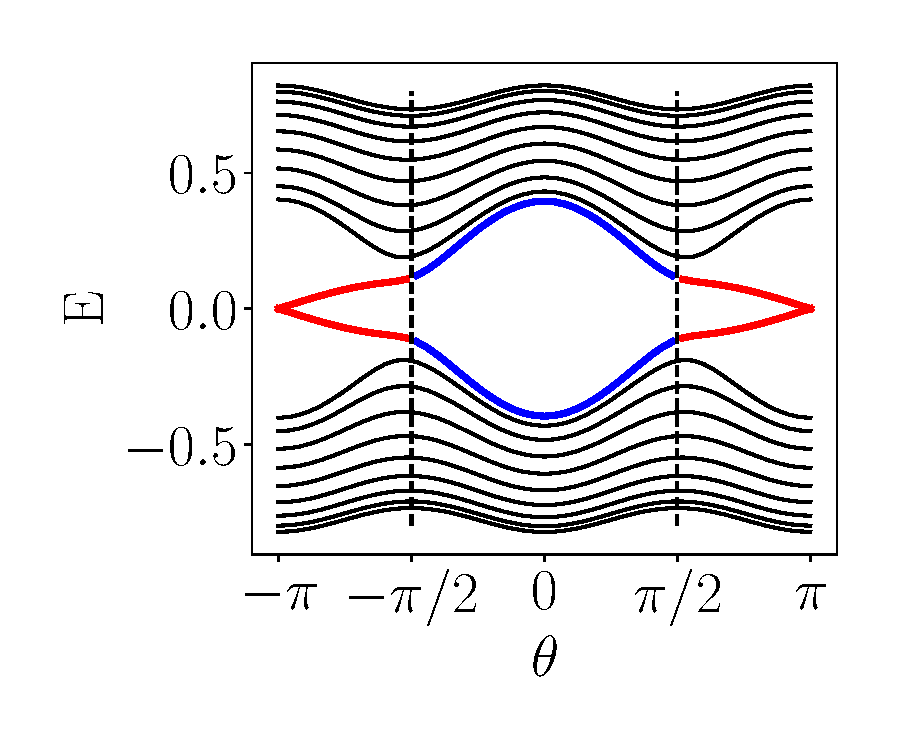
\includegraphics[width=\textwidth]{Imagenes/Shh_images/bands_shh_pump.pdf}
     \end{subfigure}\hspace*{-0.9em}
     \begin{subfigure}[b!]{0.27 \textwidth}
         \caption{}
         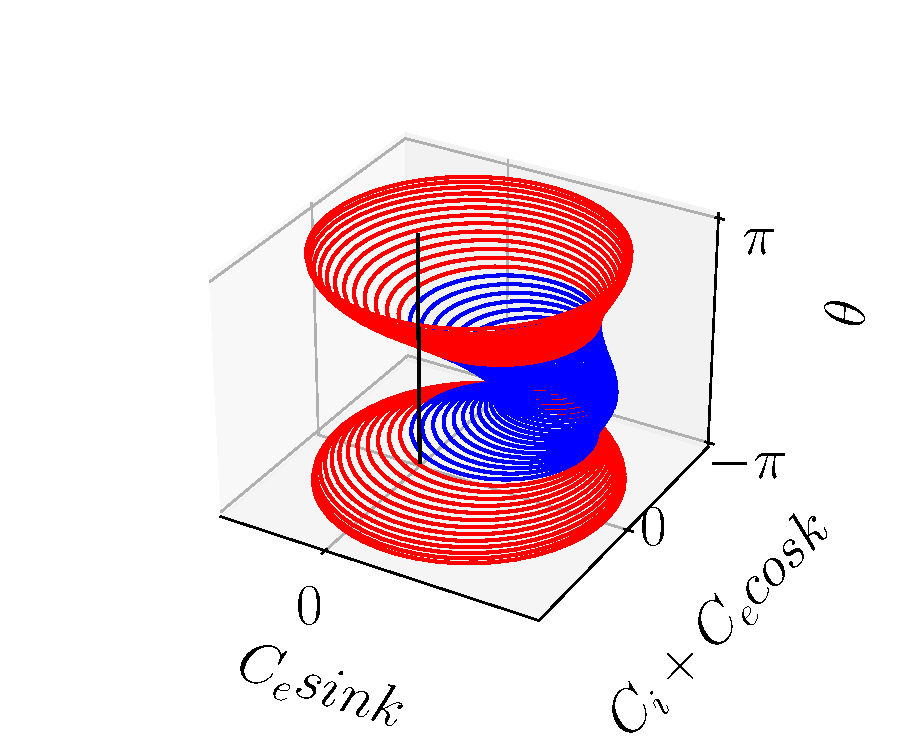
\includegraphics[width=\textwidth]{Imagenes/Shh_images/loop_pump_ssh.pdf}
     \end{subfigure}\hspace*{-0.9em}
     \begin{subfigure}[b!]{0.27 \textwidth}
         \caption{}
         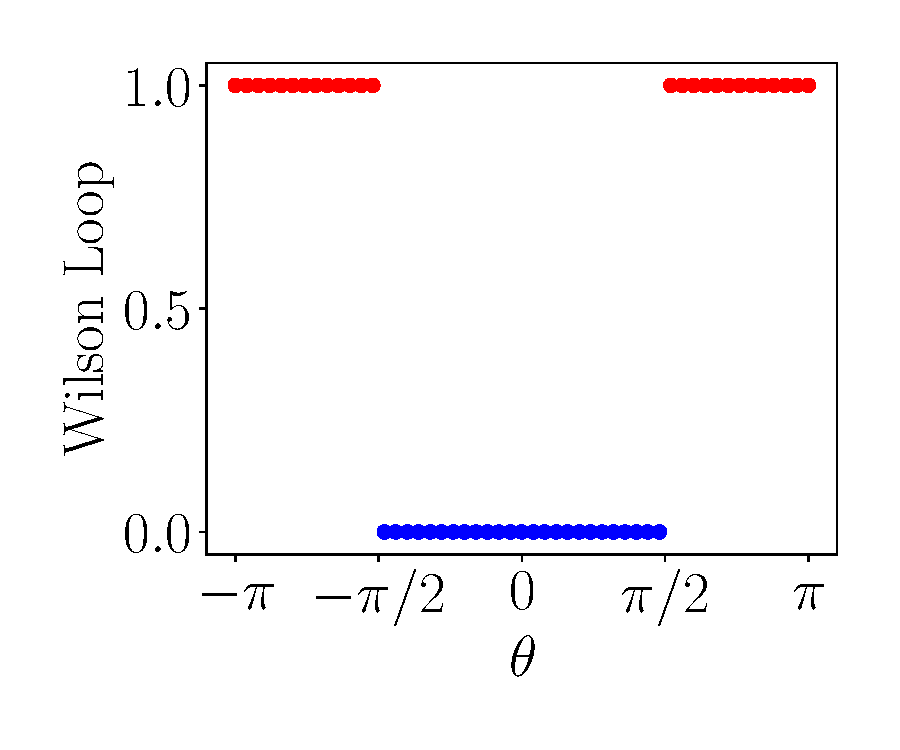
\includegraphics[width=\textwidth]{Imagenes/Shh_images/winding_shh_pump.pdf}
     \end{subfigure}\hspace*{-0.9em}
     \begin{subfigure}[b!]{0.27 \textwidth}
         \caption{}
         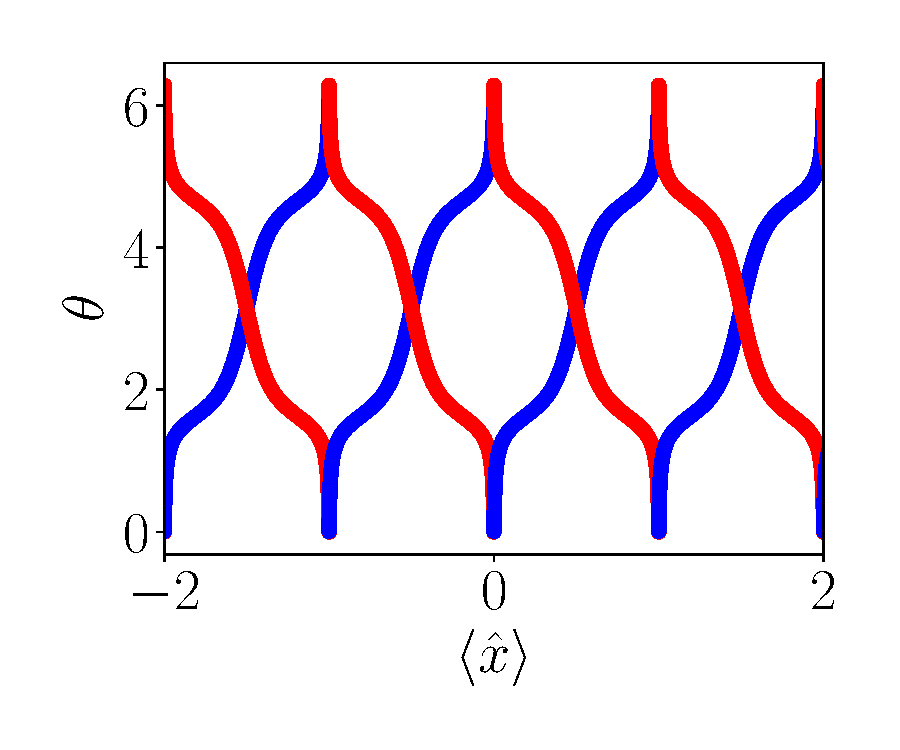
\includegraphics[width=\textwidth]{Imagenes/Shh_images/wannier_center_shh_pump.pdf}
     \end{subfigure}
     \caption{\textbf{(a)} Variación del espectro de energias conforme cambia el parametro ciclico $\theta$. \textbf{(b)} Representacion grafica del número de Winding en la fase topológica (rojo) y en la fase trivial (azul). \textbf{(c)}Fase de Berry dependiente de los parametros de salto $\gamma/\lambda$ con valor $1$ en fase topológica (rojo) y $0$ en la fase trivial (azul) .\textbf{(d)} cambio del valor esperado o centros de wannier conforme varia el parametro ciclico.}
    \label{fig:Pump_example_Results}
\end{figure}

Una de las aplicaciones mas interesantes de la fase de Berry es demostrar que el cambio lento de los parámetros temporales en un solido 1-dimensional puede generar transporte o bombeo de cargas después de recorrer un ciclo.

Recordemos que en el caso del modelo de SSH anterior teníamos parámetros que al variar mostraban cambios en los estados de la geometría estudiada, una forma de poder analizar como suceden estas transiciones de fase es a través del bombeo adiabático, haciendo variar los parámetros de salto del hamiltoniano por medio de un parámetro adiabático y cíclico.

\subsection{Modelo de Rice-Mele}

Consideremos el hamiltoniano de SSH del modelo anterior, con una pequeña modificación, los parámetros de salto variarán en el tiempo a través de un parámetro cíclico $\theta \in \left[ 0 , 2\pi\right]$ y agregaremos un termino de sitio que nos permitirá suavizar los estados de transición:

% \begin{align}
%     \nonumber\gamma \rightarrow C_{int}(\theta) = \gamma\exp(-\beta(-A \cos \theta - 1)) \; &,\;  \lambda \rightarrow C_{ext}(\theta) = \lambda \exp(-\beta( A \cos \theta - 1 )) \;,\; \\  C_{in}(\theta) = \delta \sin \theta
% \end{align}

\begin{align}
    \nonumber\gamma \rightarrow \gamma (\theta) = \gamma_0 e^{\displaystyle-\beta(-A \cos \theta - 1)} \; &,\;  \lambda \rightarrow \lambda(\theta) = \lambda_0 e^{\displaystyle-\beta( A \cos \theta - 1 )} \;,\; \\  \epsilon(\theta) = \epsilon_0 \sin \theta
\end{align}

Con $\epsilon_0$ suficientemente pequeño.

De tal forma que el nuevo modelo estará descrito por el siguiente hamiltoniano de Bloch:
\begin{equation}
    H_k(\theta) =      
     \begin{pmatrix}
            \epsilon(\theta) & \gamma(\theta) + \lambda(\theta) e^{-ik}  \\
            \gamma(\theta) + \lambda(\theta) e^{ik} & -\epsilon(\theta) \\
        \end{pmatrix} 
\end{equation}
Y el hamiltoniano en el espacio real, para una cadena con 4 celdas unitarias:
\begin{equation}
    H (\theta)= 
     \begin{pmatrix}
            \epsilon(\theta) & \gamma(\theta) & 0 & 0 & 0 & 0 & 0 & 0 \\
            \gamma(\theta) & -\epsilon(\theta) & \lambda(\theta) & 0 & 0 & 0 & 0 & 0 \\
            0 & \lambda(\theta) & \epsilon(\theta) & \gamma(\theta) & 0 & 0 & 0 & 0 \\
            0 & 0 & \gamma(\theta) & -\epsilon(\theta) & \lambda(\theta) & 0 & 0 & 0 \\
            0 & 0 & 0 & \lambda(\theta) & \epsilon(\theta) & \gamma(\theta) & 0 & 0 \\
            0 & 0 & 0 & 0 & \gamma(\theta) & -\epsilon(\theta) & \lambda(\theta) & 0 \\
            0 & 0 & 0 & 0 & 0 & \lambda(\theta) & \epsilon(\theta) & \gamma(\theta) \\
            0 & 0 & 0 & 0 & 0 & 0 & \gamma(\theta) & -\epsilon(\theta) \\
            
        \end{pmatrix}
\end{equation}

En la figura \ref{fig:Pump_example_Results} \textbf{(a)}, \textbf{(b)} y \textbf{(c)} se pueden observar diferentes formas de observar la transición de fase entre fase topológica y trivial, en fig.\ref{fig:Pump_example_Results} \textbf{(a)}, se puede ver como en el espectro de bandas el comportamiento de las energías de los estados de borde cambian de tener un gap amplio, es decir una fase trivial, a tener una brecha energética nula o una fase topológica, podemos seguir este cambio a través del numero de winding, en la fig.\ref{fig:Pump_example_Results} \textbf{(b)} como los círculos que forman la relación de dispersión pasan de rodear el origen a no hacerlo, en la fig.\ref{fig:Pump_example_Results} \textbf{(c)} se puede observar un cambio mas abrupto en la transición de fase no trivial, pues este caracteriza la fase que la ecuación de onda gana cuando se recorre un ciclo por la zona de brilluan, esto determina que hay valores en la variación temporal en los que el material ganara una fase y hay otros en los que no. Por ultimo, Si nuestro material gana una fase y traiciona de estado a estado después de en un ciclo, existe un cambio en el? La respuesta es si, a pesar de que el hamiltoniano del material no haya cambiado después de el ciclo, los eigenestados si cambiaron y esto se ve reflejado en un bombeo de cargar a través de la cadena.

\begin{figure}[h!]
    \centering
   \captionsetup[sub]{font=small}

    \begin{subfigure}[b!]{0.2 \textwidth}
        \caption*{$\theta=-\pi$}
        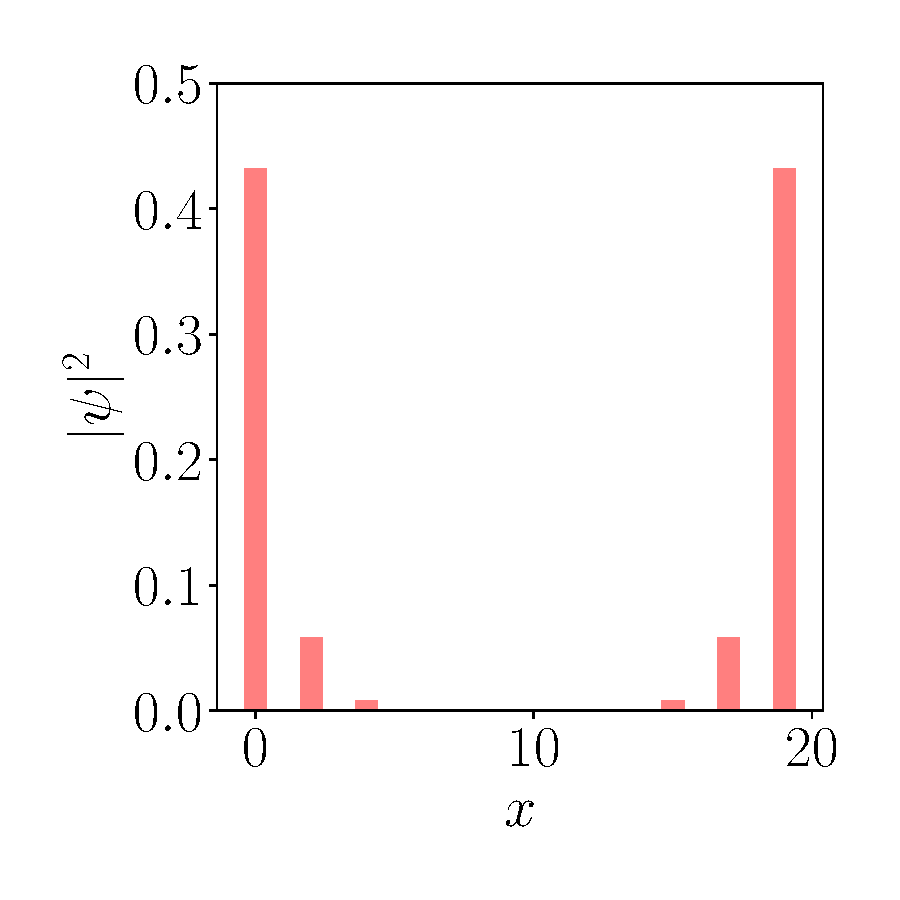
\includegraphics[width=\textwidth]{Imagenes/Shh_images/proyection_0.pdf}
    \end{subfigure}\hspace*{-0.9em}
    \begin{subfigure}[b!]{0.2 \textwidth}
        \caption*{$\theta=-\frac{\pi}{2}$}
        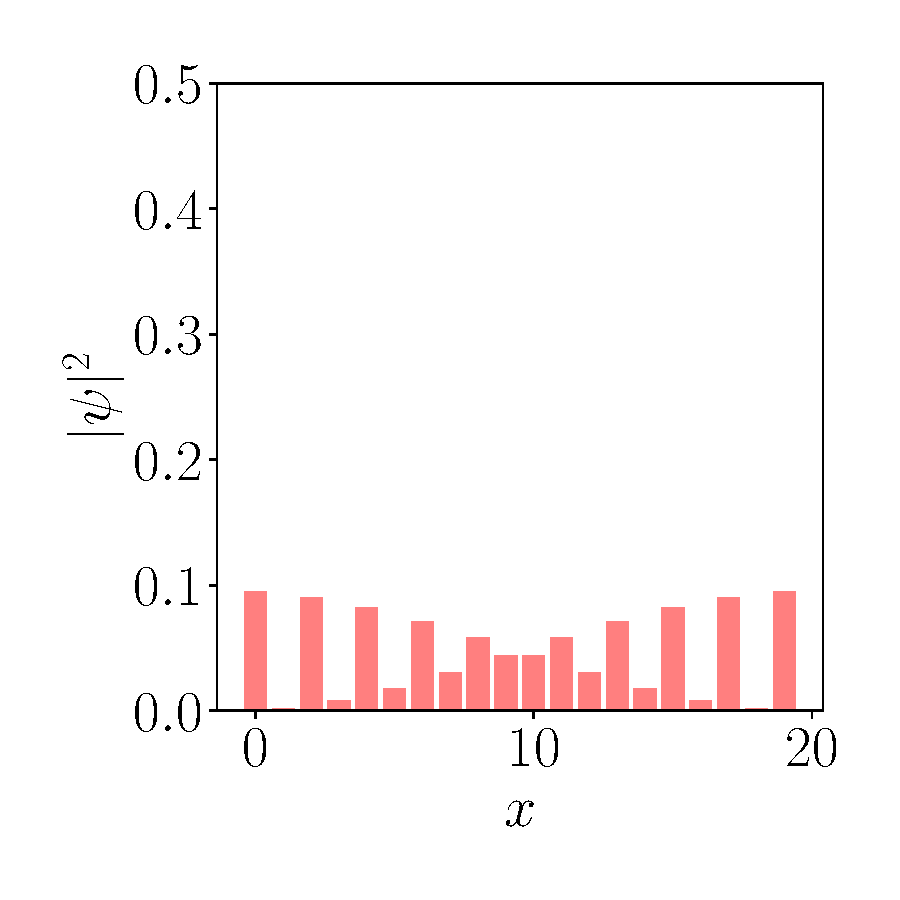
\includegraphics[width=\textwidth]{Imagenes/Shh_images/proyection_1.pdf}
    \end{subfigure}\hspace*{-0.9em}
    \begin{subfigure}[b!]{0.2 \textwidth}
        \caption*{$\theta=0$}
        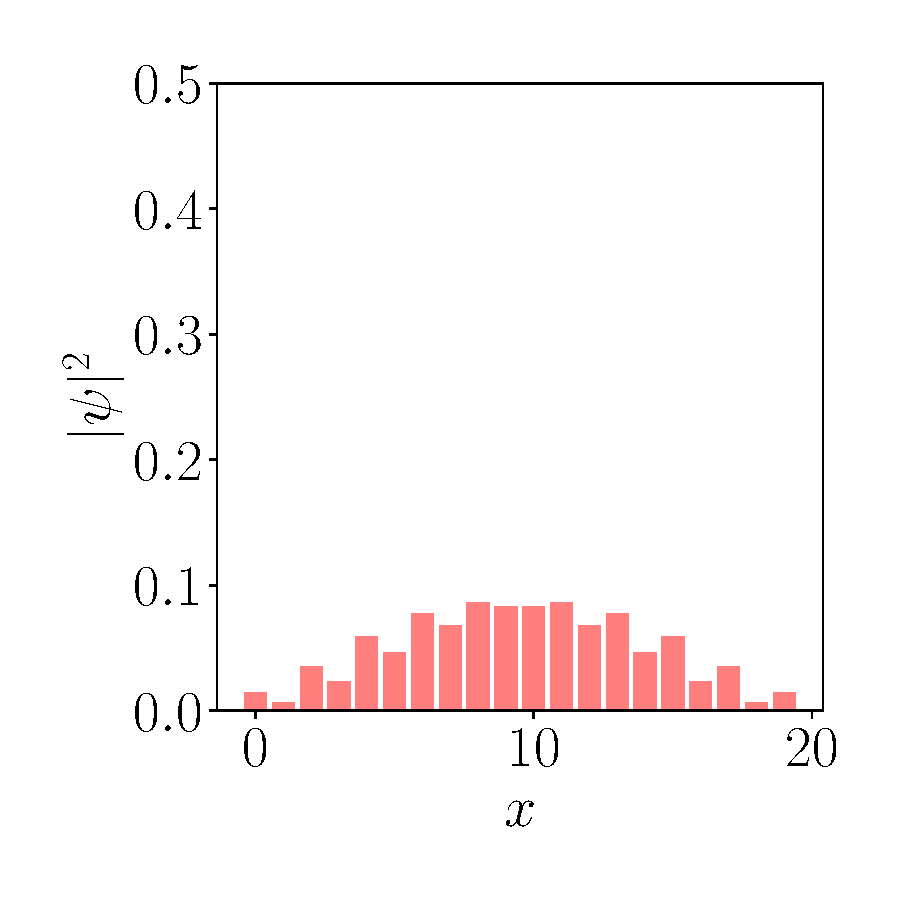
\includegraphics[width=\textwidth]{Imagenes/Shh_images/proyection_2.pdf}
    \end{subfigure}\hspace*{-0.9em}
    \begin{subfigure}[b!]{0.2 \textwidth}
        \caption*{$\theta=\frac{\pi}{2}$}
        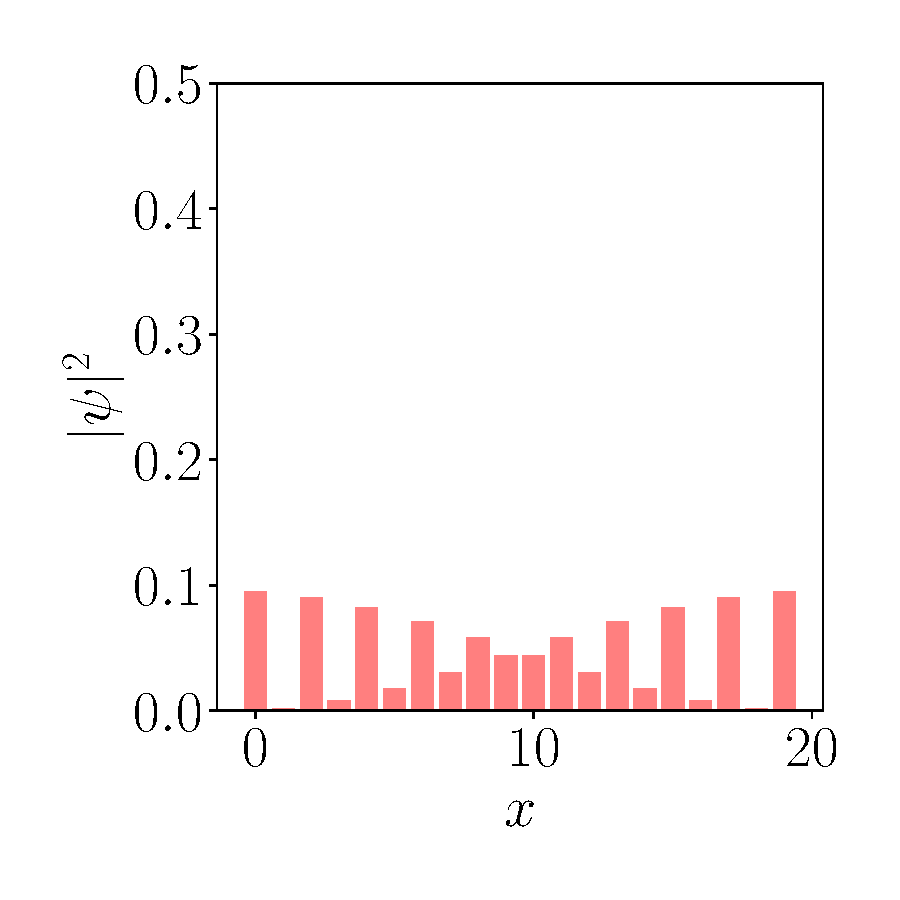
\includegraphics[width=\textwidth]{Imagenes/Shh_images/proyection_3.pdf}
    \end{subfigure}\hspace*{-0.9em}
    \begin{subfigure}[b!]{0.2 \textwidth}
        \caption*{$\theta=\pi$}
        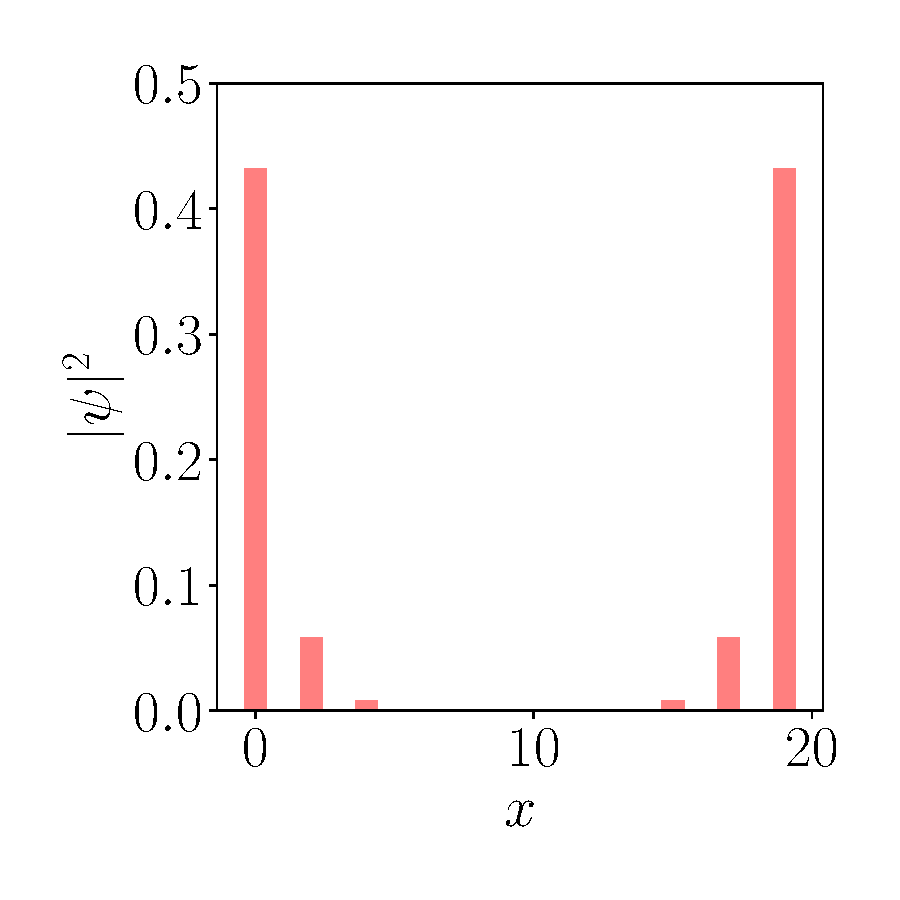
\includegraphics[width=\textwidth]{Imagenes/Shh_images/proyection_4.pdf}
    \end{subfigure}
       \caption{Proyección de los estados correspondientes a las energias negativas mas cernas a los estados de Fermi para distintos valores de $\theta \in [-\pi, \pi]$. }
    \label{fig:pump_RM_proyection}
\end{figure}

Una forma de estudiar esta cuestión es a través de hacer un seguimiento de los centros de wannier de cada celda, si existe un desplazamiento de este centro de celda a celda, la fase que gana nuestro sistema después de un ciclo, se puede interpretar como el desplazamiento de cargas de una celda a otra lo que denotaría que existe un bombeo y como vimos en el capitulo anterior, la corriente generada por este bombeo propicia un estado de polarización en el material, el cual se puede observar cuando proyectamos los estados de las energías centrales de \ref{fig:Pump_example_Results} \textbf{(a)} en el espacio real, fig(\ref{fig:pump_RM_proyection}).


\section{Fractales (Sierpinsky Carpet)}
\label{sc:Fractales}

\begin{figure}[h!]
     \centering
    \captionsetup[sub]{font=small}

     \begin{subfigure}[b!]{0.27 \textwidth}
         \caption{}
         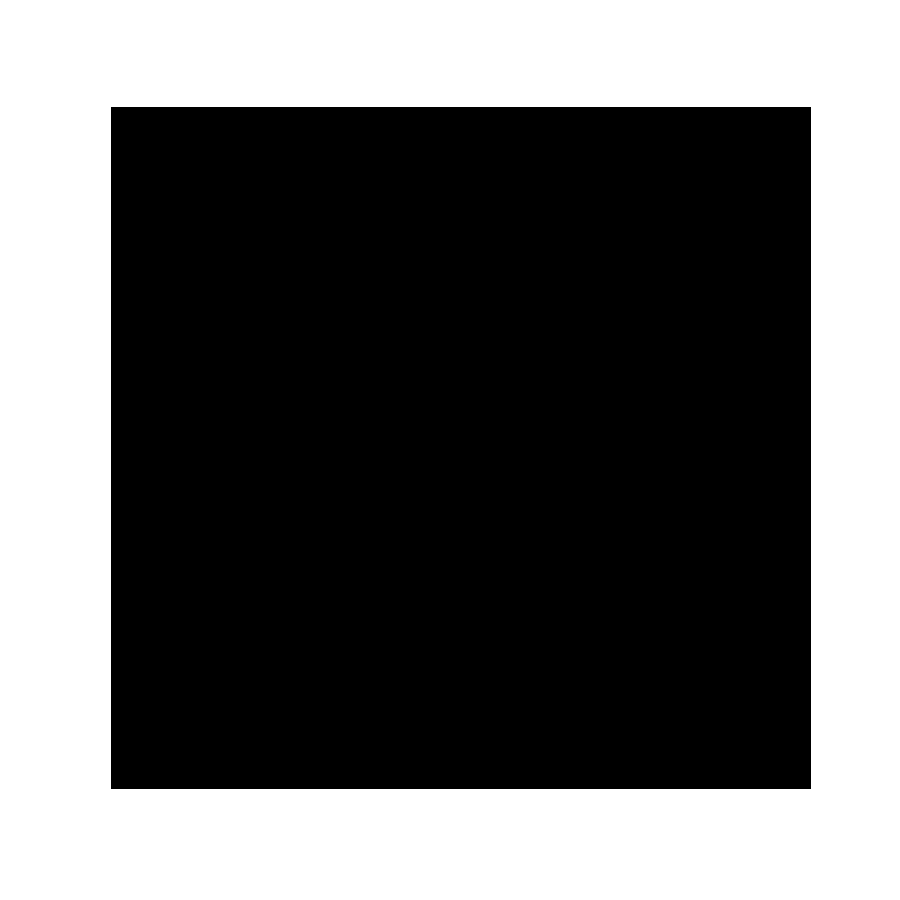
\includegraphics[width=\textwidth]{Imagenes/Fractal/sierpinski_carpet_1.pdf}
     \end{subfigure}\hspace*{-0.9em}
     \begin{subfigure}[b!]{0.27 \textwidth}
         \caption{}
         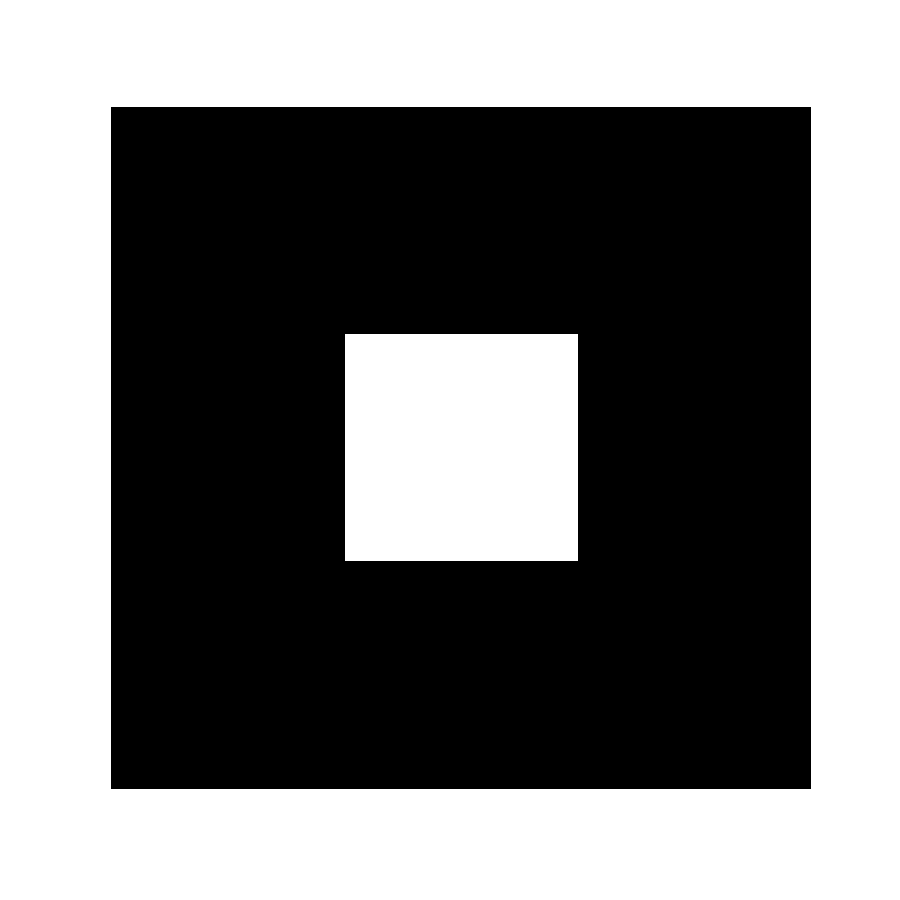
\includegraphics[width=\textwidth]{Imagenes/Fractal/sierpinski_carpet_2.pdf}
     \end{subfigure}\hspace*{-0.9em}
     \begin{subfigure}[b!]{0.27 \textwidth}
         \caption{}
         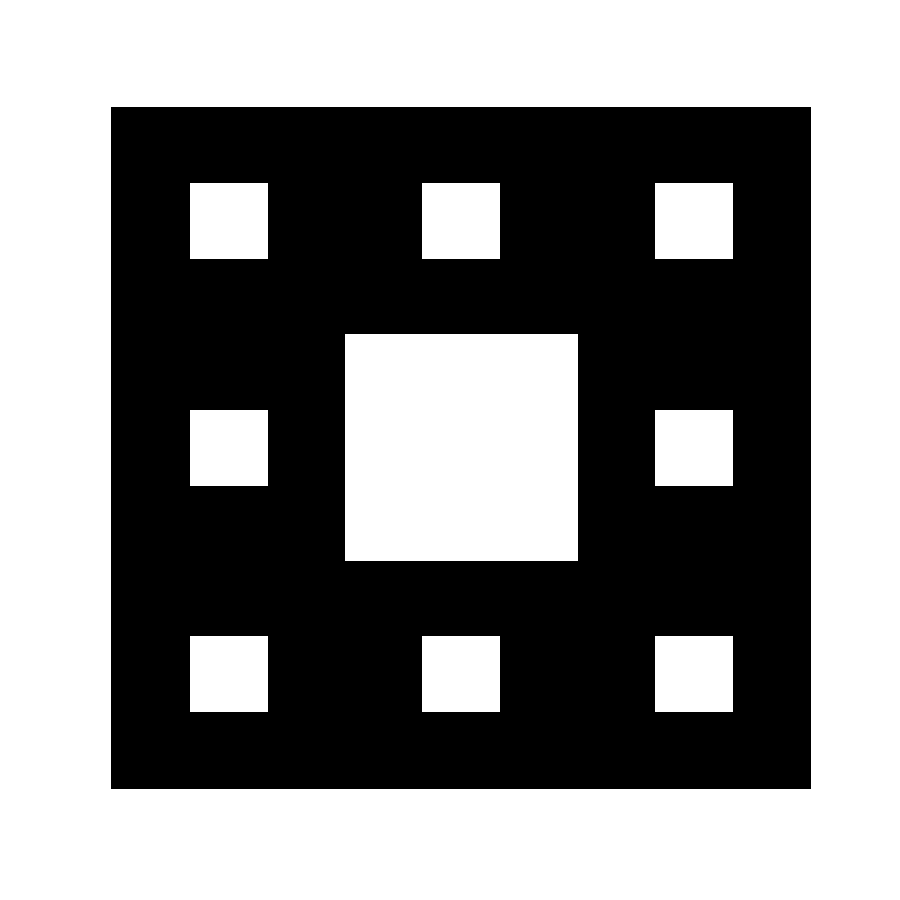
\includegraphics[width=\textwidth]{Imagenes/Fractal/sierpinski_carpet_3.pdf}
     \end{subfigure}\hspace*{-0.9em}
     \begin{subfigure}[b!]{0.27 \textwidth}
         \caption{}
         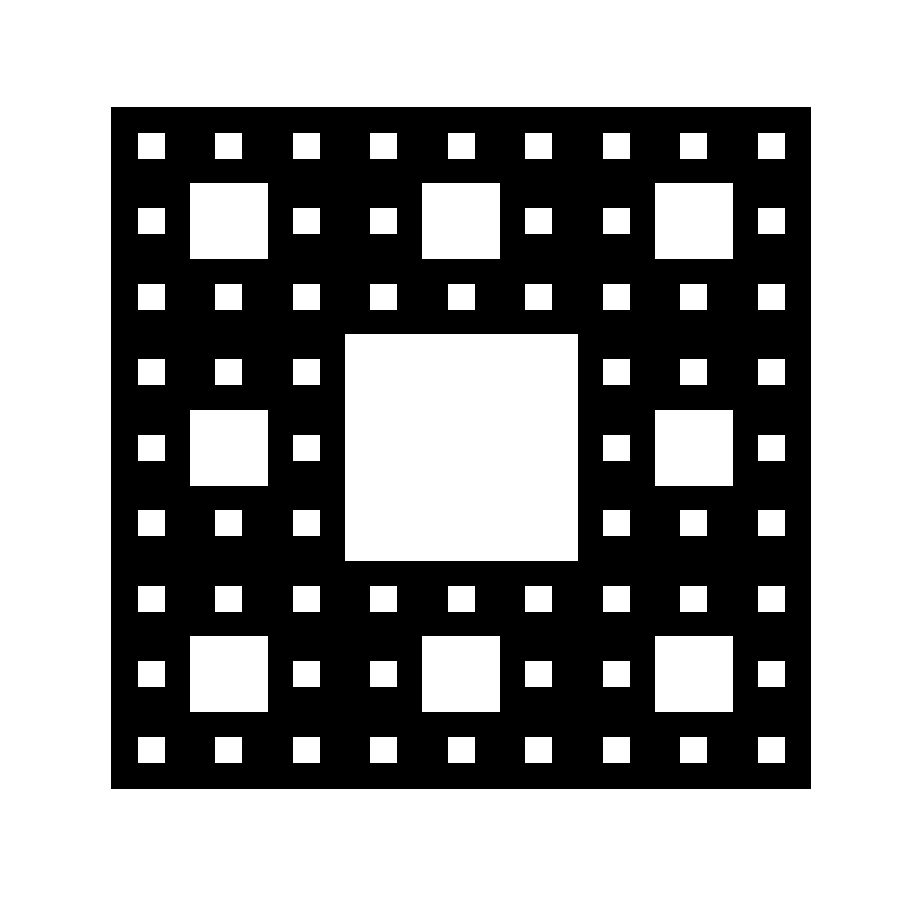
\includegraphics[width=\textwidth]{Imagenes/Fractal/sierpinski_carpet_4.pdf}
     \end{subfigure}
        \caption{Procedimiento para generar una red o alfombra de Sierpinski, conforme aumentan las iteraciones, \textbf{(a)} $n=0$, \textbf{(b)} $n=1$, \textbf{(c)} $n=2$,\textbf{(d)} $n=3$.}
        \label{fig:Fractals}
\end{figure}

Hemos observado que las propiedades electrónicas de los materiales que estudiamos depende casi totalmente de las propiedades geométricas que lo definen. La relaciones y la separación entre los estados de borde y de bulto, permiten construir estados de polarización así como hacer un seguimiento del bombeo de las cargas en parámetros cíclicos. Pero, que pasaría si las geometrías de los materiales, tienen mas de un borde o la idea de la relación cuerpo-borde o área y perímetro se pierden? 

Una de las geometrías mas interesantes que cumplen estas características son las fractales, construcciones geométricas que se basan en la realización iterativa y poseen propiedades como la dimensión no entera, y la autosemejanza. Para los fines de este trabajo nos concentraremos en la alfombra de Sierpinski, el cual es un fractal descrito por el matemático polaco Waclaw Sierpinski en 1916. Se construye dividiendo un cuadrado en otros nueve de lado 1/3 del original y eliminando el cuadrado que ocupa la posición central, repitiendo este proceso en cada uno de los cuadrados que
quedan, indefinidamente.

En cada iteración el numero de huecos cuadrados va aumentando de la siguiente manera (fig \ref{fig:Fractals}):
\begin{equation}
    1,\; 8, \; 8^2,\;\dots\; 8^n
\end{equation}
respectivamente, cada lado del cuadrado escala como un tercio del anterior:
\begin{equation}
    1,\; \frac{1}{3}, \; \left( \frac{1}{3} \right)^2,\;\dots\; \left( \frac{1}{3} \right)^n
\end{equation}
como resultado se obtiene así un objeto geométrico “hueco” de área nula pero con perímetro infinito. Al calcular su dimensión obtenemos:

\begin{equation}
    D = \frac{log N(r)}{log 1/r} = \frac{log 8^n}{log 3^n} = 1.8927
\end{equation}

Donde $N(r)$ es el numero de figuras que se generan por iteración y $r$ es la relación de escala de cada lado por cada iteración.

Los fractales considerados en este trabajo están definidos en un numero finito de iteraciones, además que en la construcción, como se vera en el próximo capitulo, el tamaño de las figuras que conforman el fractal crecen como múltiplos de la celda unitaria, por lo cual no hay una dilución del área solo existe respecto al tamaño final, esto implica que en este trabajo que los fractales considerados en este trabajo sean fractales aproximados.

